\chapter{Results}

\section{TDC}
The TDC was simulated in Cadence Virtuoso using the Spectre simulator. The test bench (TB) is that of figure \ref{fig:TB_TDC_Schematic}, where the reference input signal is connected
to a square wave voltage source with a frequency of 100 MHz and a 50\% duty cycle, the other input (feedback) is connected to a similar source but with a frequency of either 100.6 MHz
or 99.4 MHz depending on whether a positive or negative phase difference is to be measured. Both of these cases simulate conditions that would occur in a PLL when the DCO frequency is
slightly higher or lower than the reference frequency, respectively. The outputs of the TDC are connected to a load capacitance of 5 fF to simulate the effect of the subsequent DLF.

\begin{figure}[H]
    \centering
    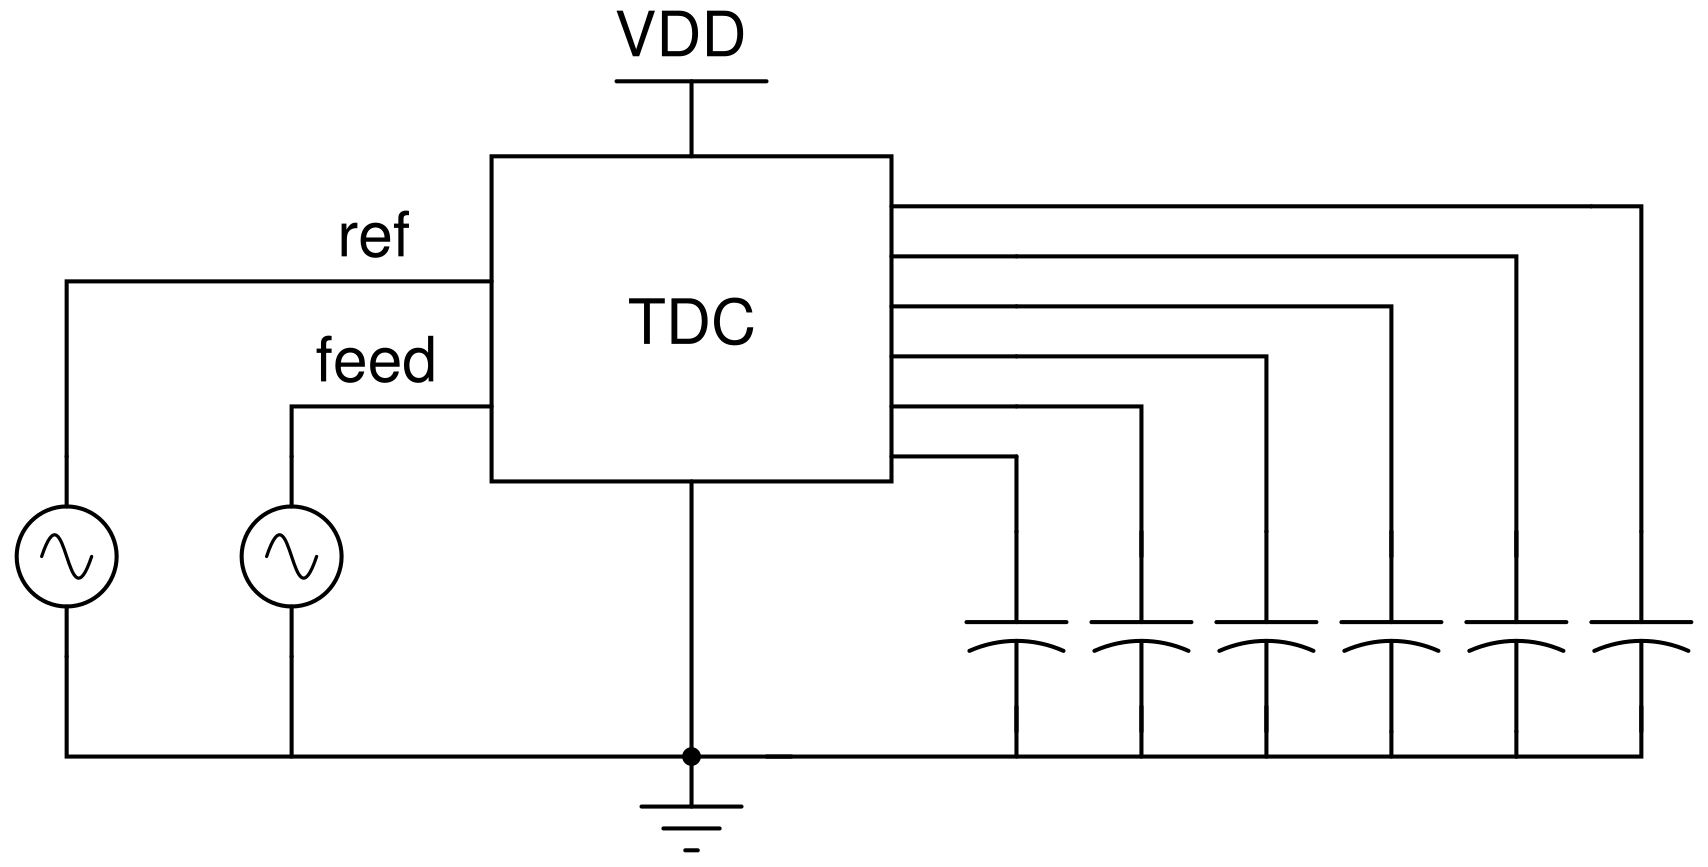
\includegraphics[width=0.7\textwidth]{figures/TB_TDC.png}
    \caption{Test bench schematic for the TDC.}
    \label{fig:TB_TDC_Schematic}
\end{figure}

The transient simulation of the TDC is separated in two parts, one for the forward path TDC and the other for the backward path TDC. Figures \ref{fig:TDC_TRAN_fwd} and \ref{fig:TDC_TRAN_bwd} show
the transient simulation results for the forward and backward path TDCs, respectively. The top two waveforms are the reference and feedback input signals, while the bottom waveforms are the TDC outputs.
The simulation is run for a total of 1.9 $\mu$s, where the first 0.3 $\mu$s is a settling time to allow the DLL to reach a steady state before measurements are taken. The next 1.6 $\mu$s are used for measurements,
allowing 10 cycles for each code.

\begin{figure}[H]
    \centering
    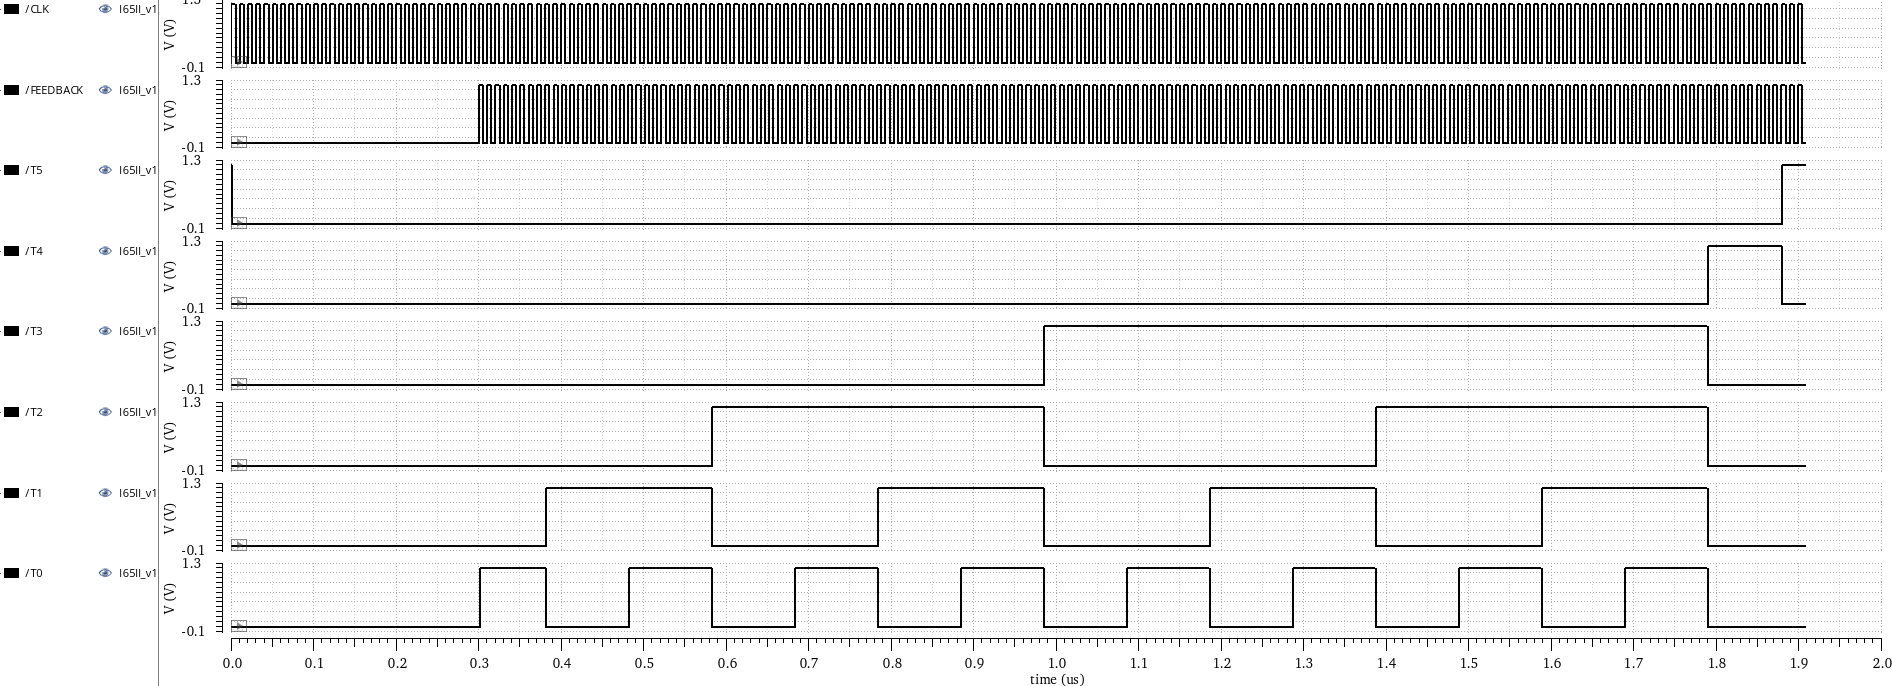
\includegraphics[width=1\textwidth]{figures/TDC_TRAN_fwd.png}
    \caption{Transient simulation results for the forward path (TT).}
    \label{fig:TDC_TRAN_fwd}
\end{figure}

\begin{figure}[H]
    \centering
    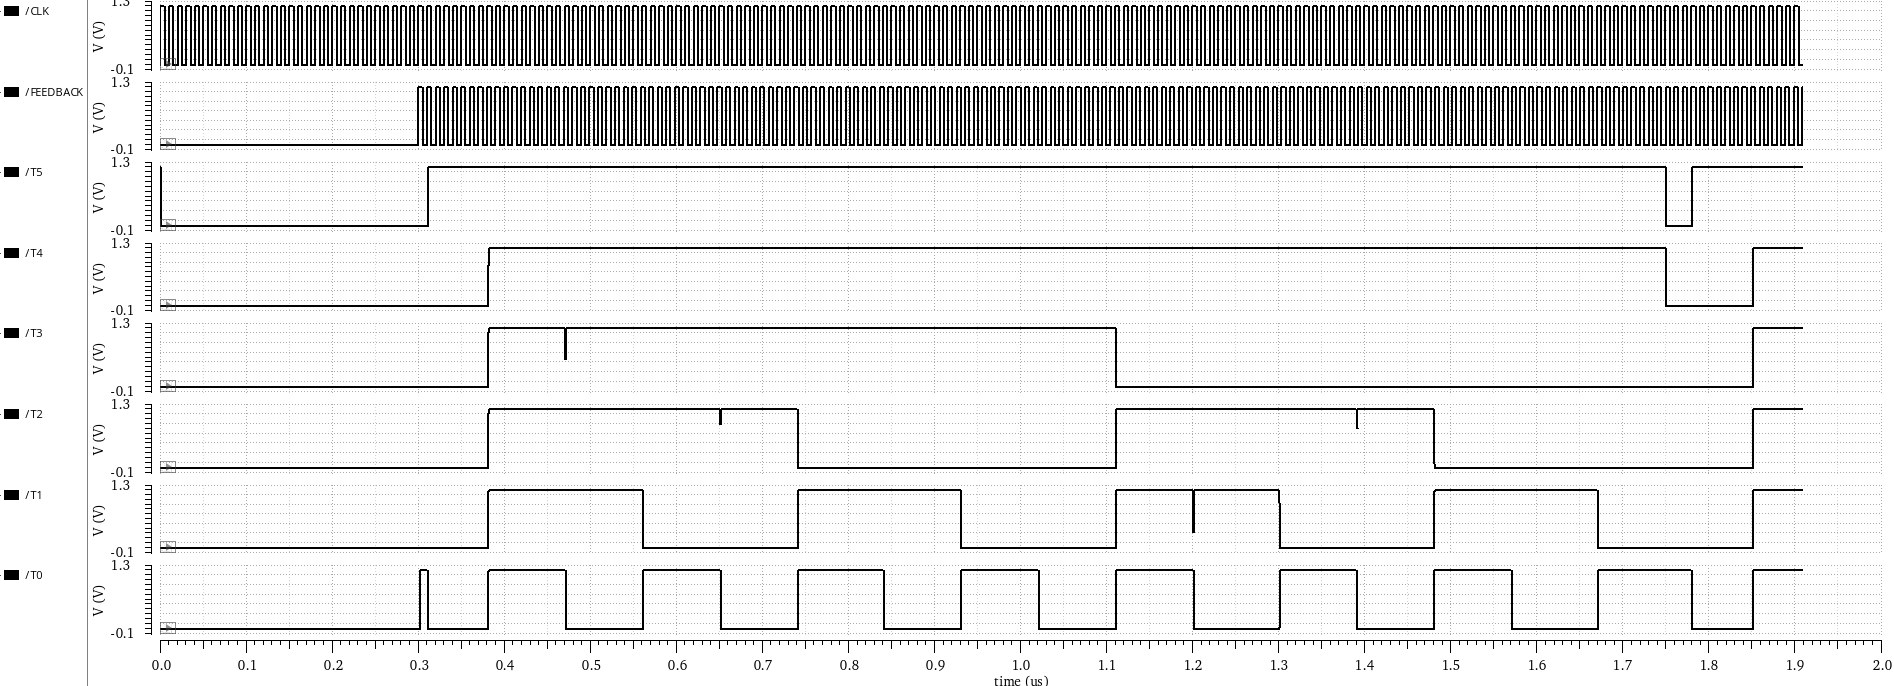
\includegraphics[width=1\textwidth]{figures/TDC_TRAN_bwd.png}
    \caption{Transient simulation results for the backward path (TT).}
    \label{fig:TDC_TRAN_bwd}
\end{figure}

The measured conversion time (defined in chapter 2 as the minimum time required for the TDC to convert an input time interval into a digital word) is found to be 687.5 ps for the typical corner (TT). From the
transient results the output characteristic of the TDC can be extracted by measuring the output code at a given delay time between the reference and feedback signals.

The output characteristic of the TDC for the typical corner is shown in figure \ref{fig:TDC_Transfer_Characteristic}, where the output is seen to increase linearly with the phase difference between the
reference and feedback signals. The red blue line is the actual output characteristic while the red dotted line is the best straight line fit. The TDC is seen to have a resolution of 625 ps and a dynamic
range of 19.687 ns. Notice that this is very similar to a PFD with a maximum phase difference of almost two full cycles but without a dead zone.

\begin{figure}[H]
    \centering
    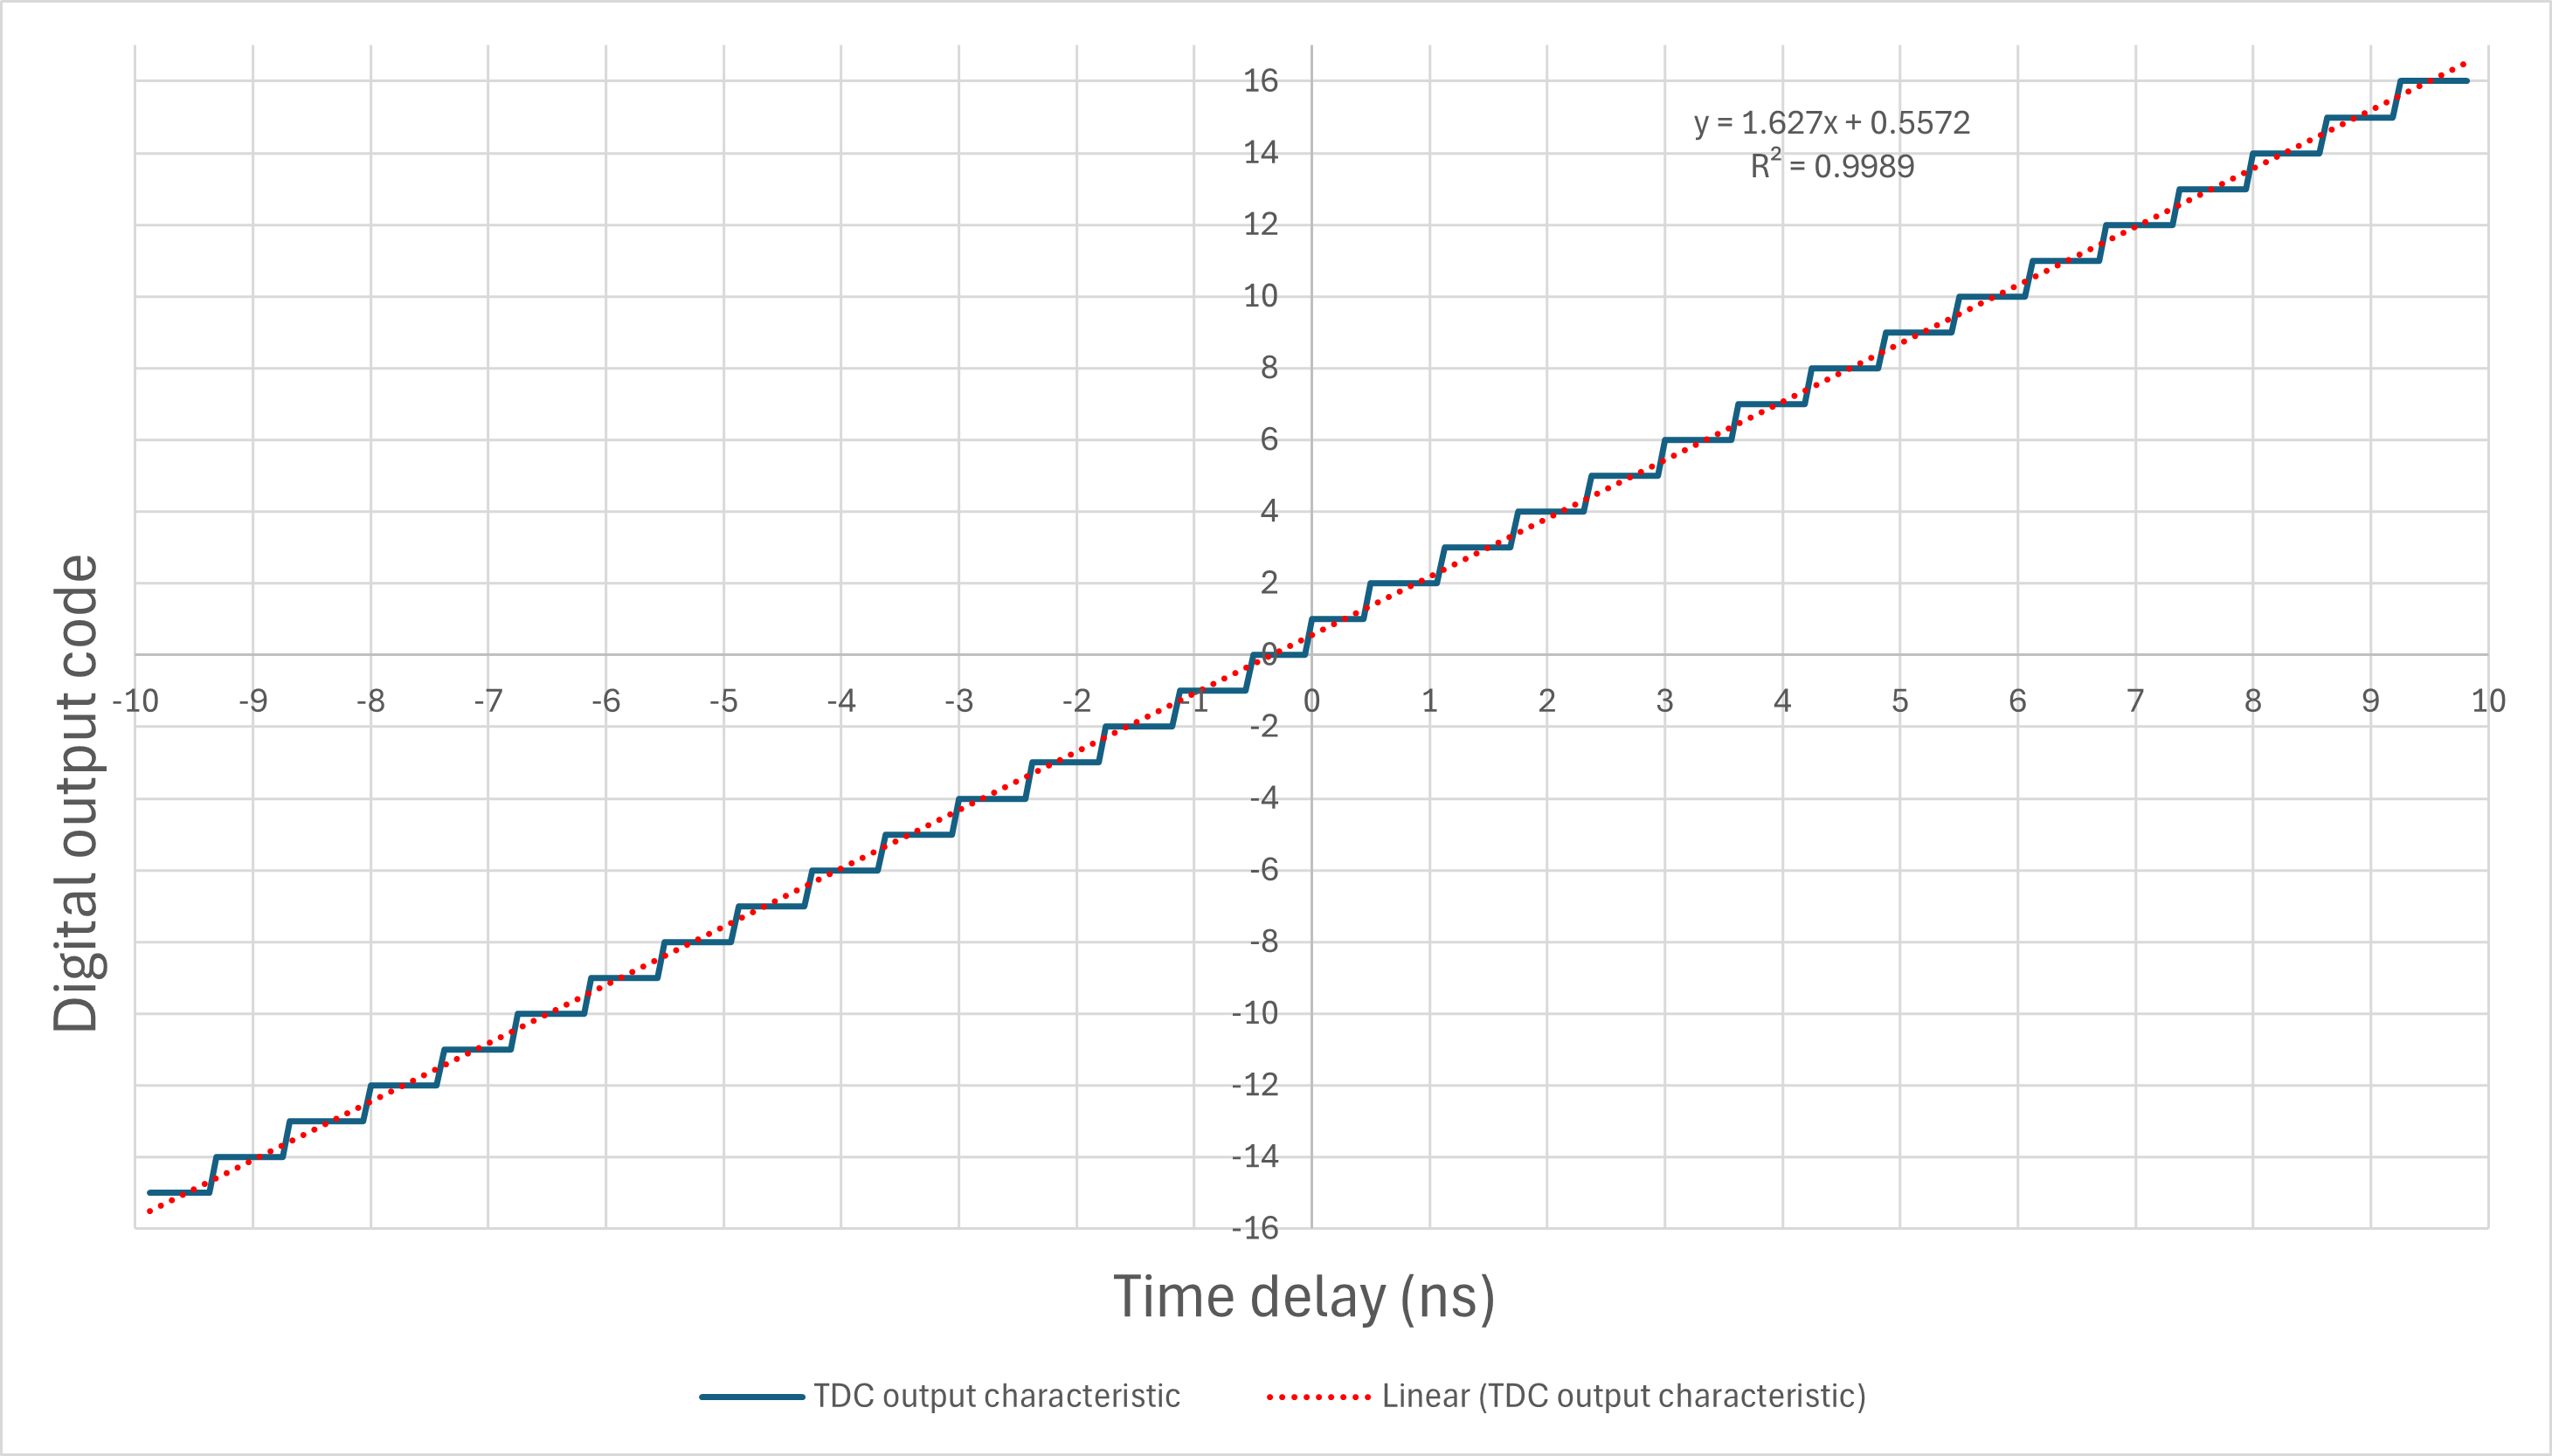
\includegraphics[width=1\textwidth]{figures/TDC_output_characteristic_result.png}
    \caption{TDC Transfer Characteristic for the TT corner.}
    \label{fig:TDC_Transfer_Characteristic}
\end{figure}

From the output characteristic, the gain of the TDC can be calculated as the slope of the best fit line, which is found to be 1.627. The linearity is calculated with the best straight line fit method,
arriving at a DNL of -0.11 LSB and INL of 0.39 LSB.

Figure \ref{fig:DLL_output_PVT} shows the output of the TDC's DLL for seven different corners (TT\_60, SS\_120, SS\_-40, FF\_120, FF\_-40, FS\_60, SF\_60).
The DLL is seen to be able to lock in all corners, with a lock time of approximately 100 ns.

\begin{figure}[H]
    \centering
    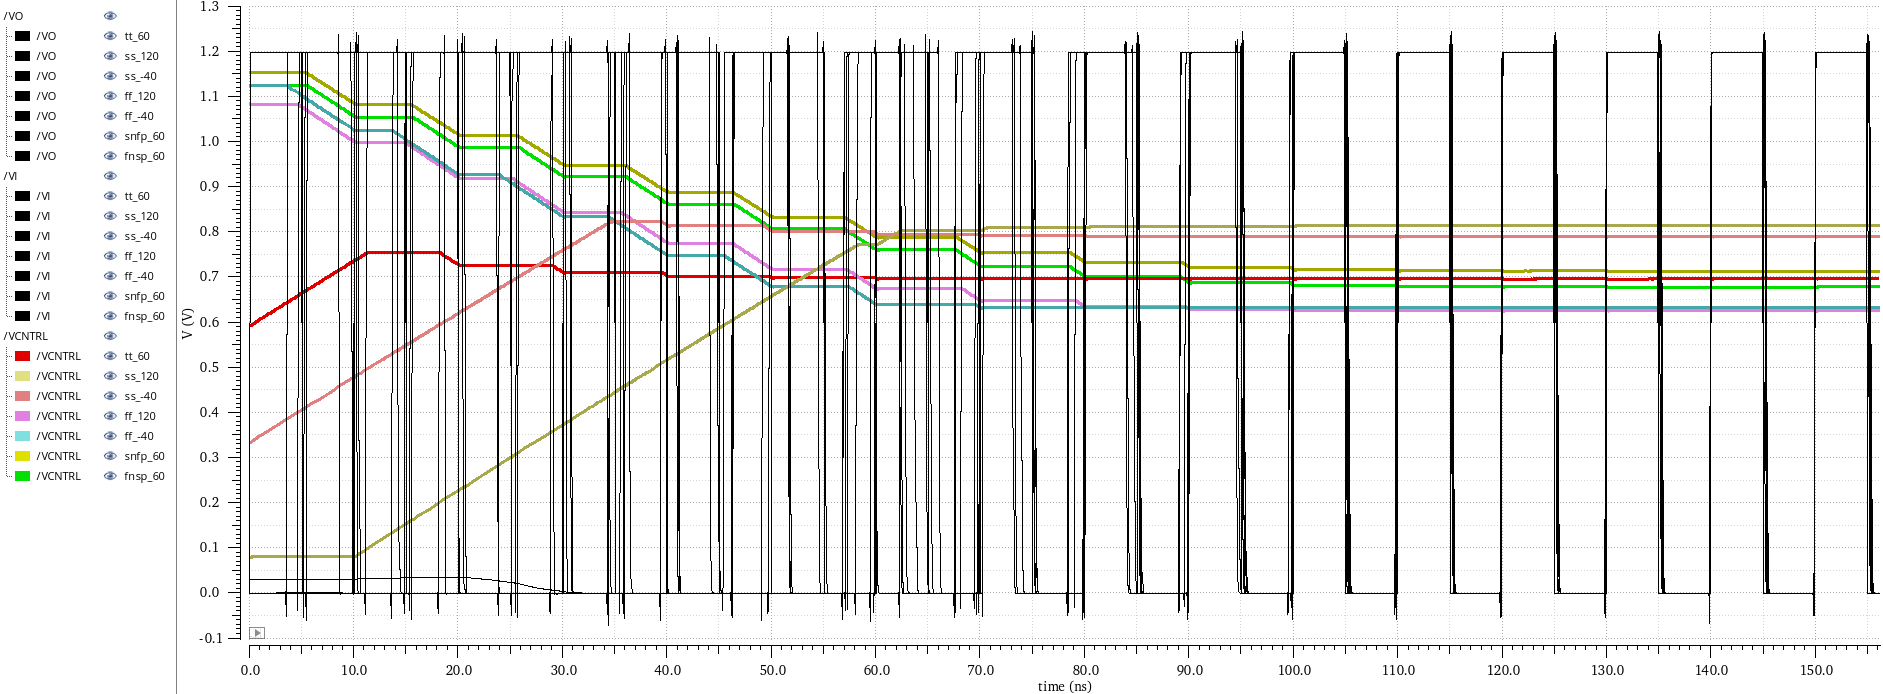
\includegraphics[width=1\textwidth]{figures/DLL_PVT2.png}
    \caption{DLL output for different PVT corners.}
    \label{fig:DLL_output_PVT}
\end{figure}

Table \ref{tab:TDC_performance_summary} summarizes the performance of the TDC and compares it with other recent works.

\begin{table}[H]
    \centering
    \caption{Performance summary of the proposed TDC and comparison with the literature.}
    \label{tab:TDC_performance_summary}
    \begin{tabular}{|c|c|c|c|}
        \hline
        Parameter & This Work & \cite{MohammadAmin2022} & \cite{Meng2025}\\
        \hline
        Technology & 65 nm CMOS & 65 nm CMOS & 28 nm CMOS \\
        Supply Voltage & 1.2 V & 1 V & 0.95 \\
        Number of bits & 4 & 7 & 10 \\
        Resolution & 625 ps & 1.7 ps & 0.39 ps\\
        Dynamic Range & 19.687 ns & 220 ps & 625 ps \\
        Conversion Time & 687.5 ps & Not reported &  Not reported \\
        DNL (LSB) & -0.11 & 1.03 & Not reported \\
        INL (LSB) & 0.39 & 1.33 & 0.27 \\
        Power Consumption & 360.54 $\mu$W & 450 $\mu$W & 14.83 mW \\
        \hline
    \end{tabular}
\end{table}

\section{DCO}
The DCO was simulated only on the nominal corner because there wasn't any PVT models available for the inductor used in the LC tank in the PDK.

Figure \ref{fig:DCO_TRAN} shows the transient simulation results for the DCO for both cases of control word (maximum and minimum frequency). The maximum frequency is found to be
8.54 GHz while the minimum frequency is 7.42 GHz, giving a tuning range of 1.08 GHz (this is taking into account a parasitic capacitance of 50 fF from a layout routing). The simulation
is run for a total of 100 ns which allows for enough cycles of the DCO to achieve steady state.

\begin{figure}[H]
    \centering
    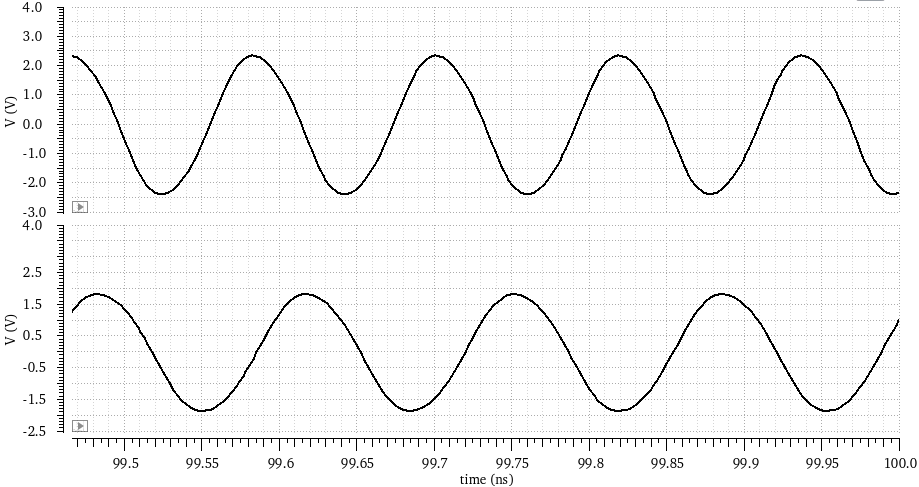
\includegraphics[width=1\textwidth]{figures/DCO_TRAN.png}
    \caption{Differential output waveform of the DCO. Maximum and minimum frequency cases.}
    \label{fig:DCO_TRAN}
\end{figure}

The DCO characteristic of figure \ref{fig:DCO_characteristic} is obtained by analyzing the periodic steady state (PSS) of the output waveform. The DCO gain is found to be 36.2 MHz/LSB.

\begin{figure}[H]
    \centering
    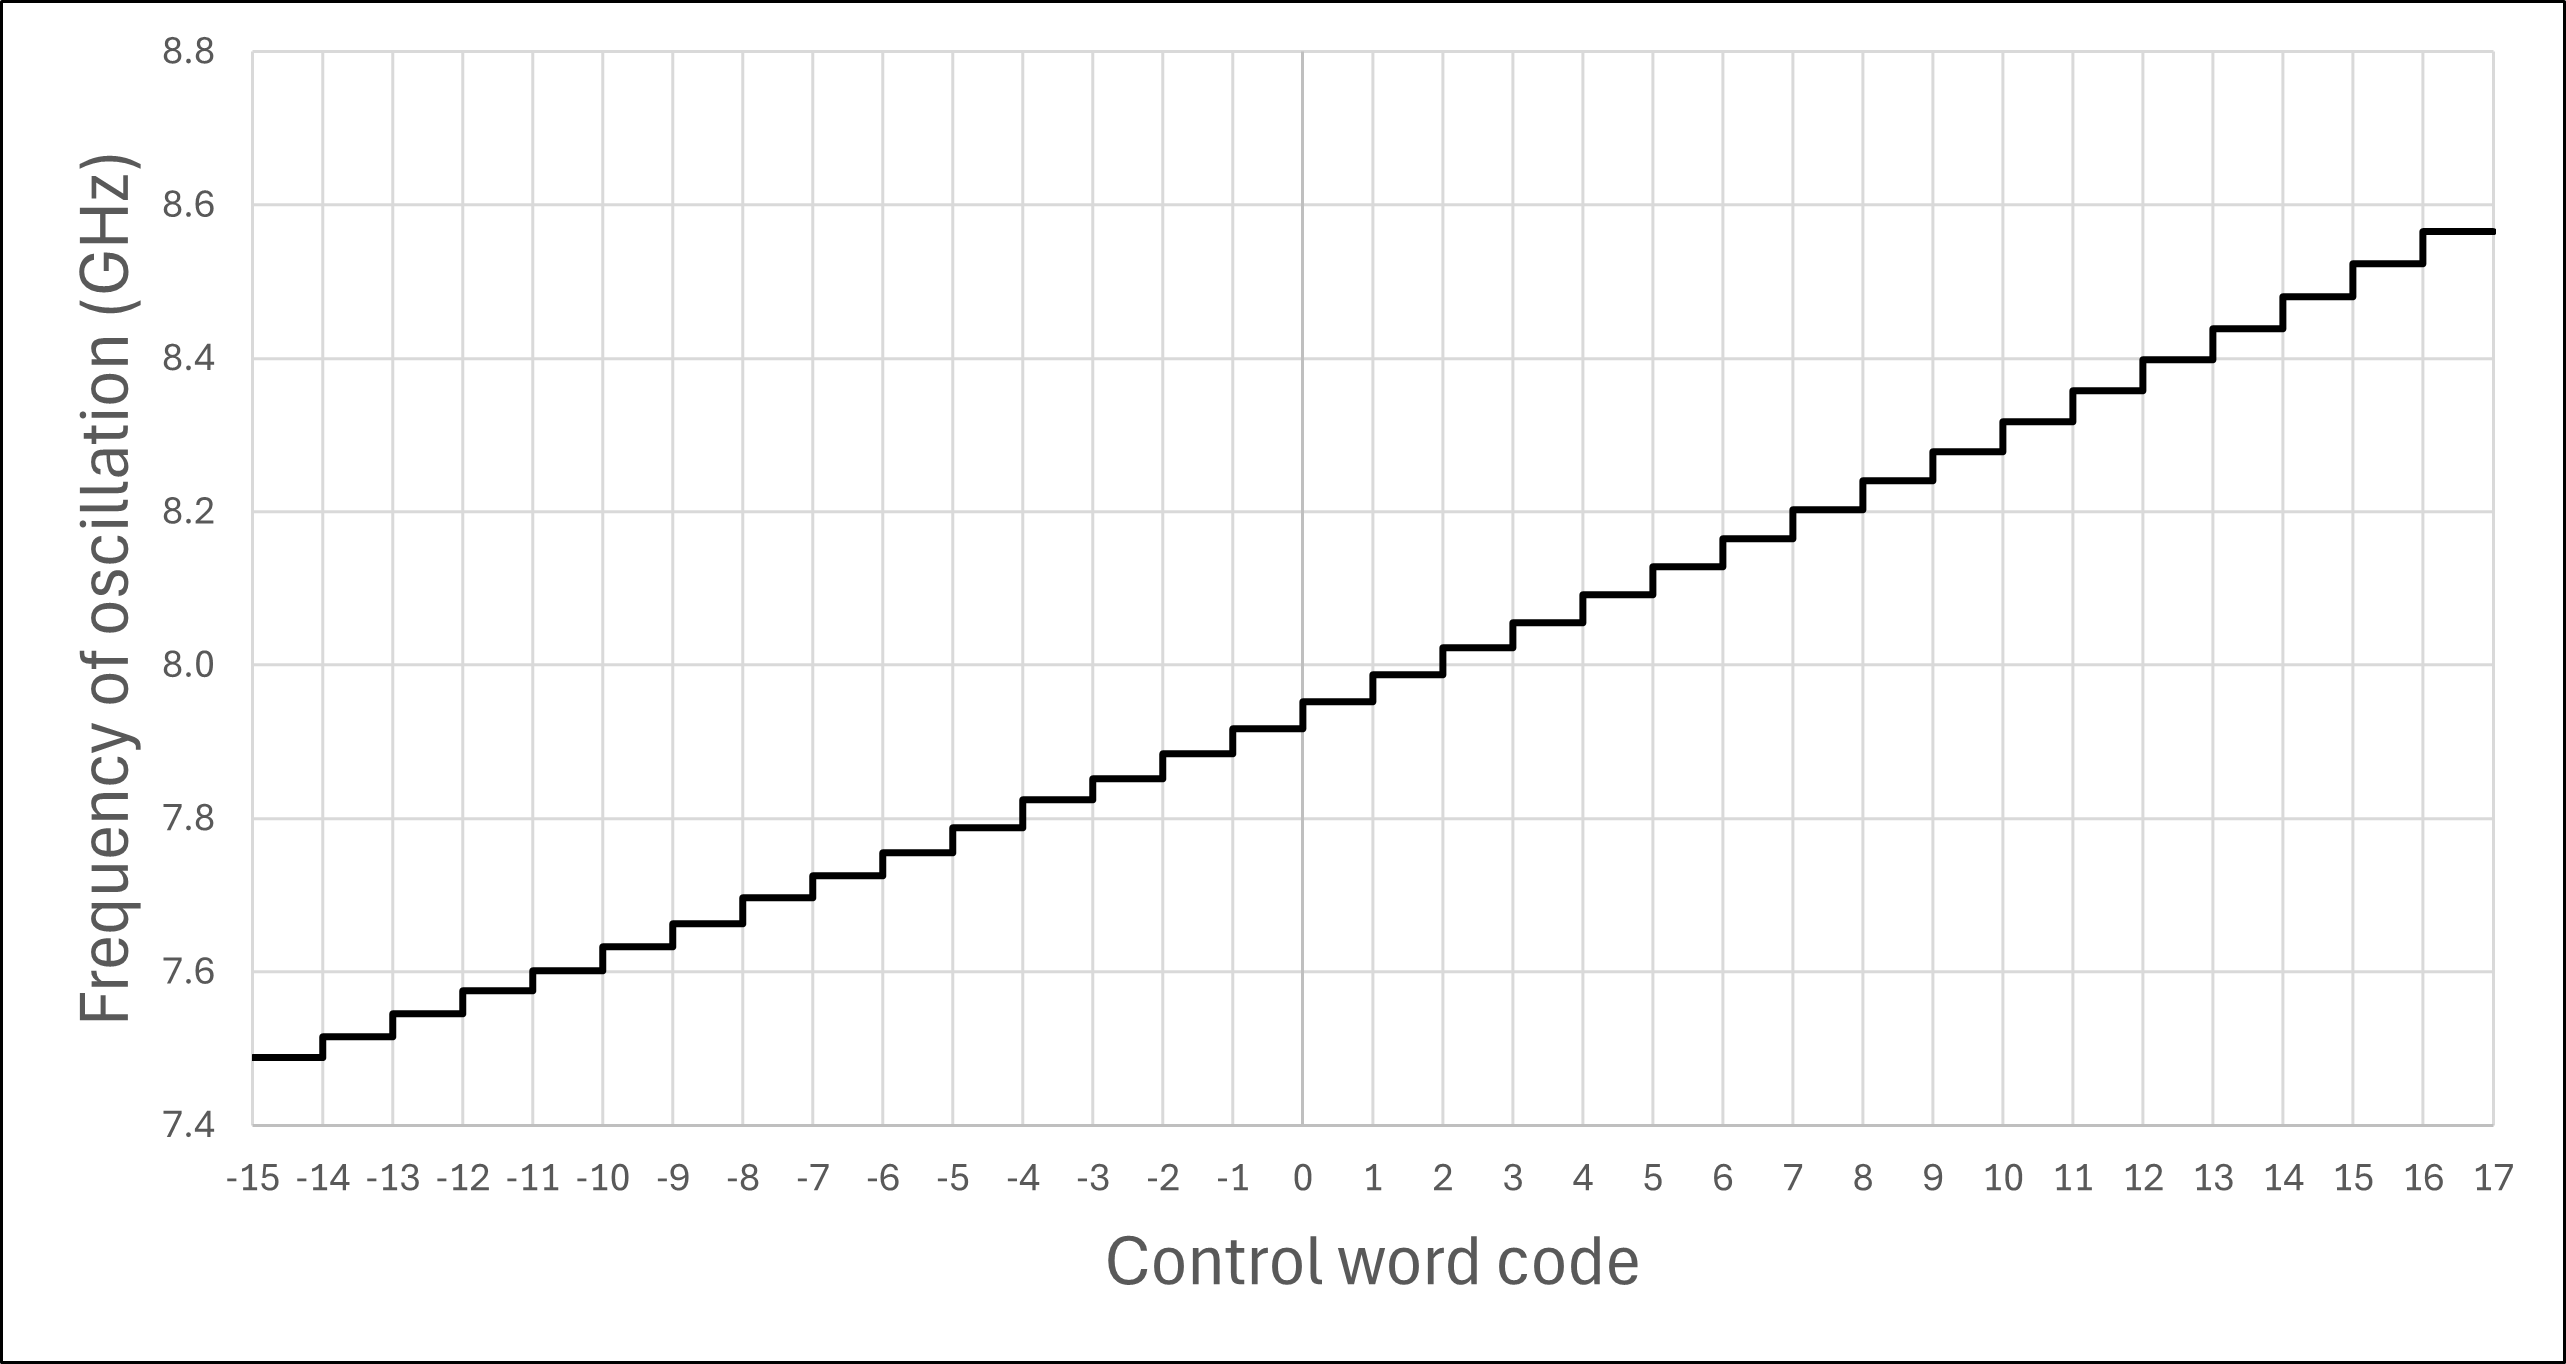
\includegraphics[width=1\textwidth]{figures/DCO_characteristic.png}
    \caption{DCO characteristic.}
    \label{fig:DCO_characteristic}
\end{figure}

The phase noise of the DCO is simulated using the periodic noise (PNoise) analysis and the first 30 harmonics. Figure \ref{fig:DCO_phase_noise} shows the
phase noise response at the center frequency of 7.92 GHz, where the phase noise is found to be -79.62 dBc/Hz at a 100 KHz sideband (or -104.17 dBc/Hz at 1 MHz) which is
a similar performance as the quadrature DCO presented by X. Chen et.al. in \cite{DCO_Chen2023}.

\begin{figure}[H]
    \centering
    \includegraphics[width=1\textwidth]{figures/DCO_phase_noise.png}
    \caption{Phase noise of the DCO at 7.92 GHz.}
    \label{fig:DCO_phase_noise}
\end{figure}

\noindent\rule{\textwidth}{1pt}